\documentclass{article}
\usepackage{graphicx}
%permite ecribir acentos directamente
\usepackage[utf8]{inputenc}
% Esto es para que el LÁTEX sepa que el texto está en español, se agrega el ingles para el paquete de gráfico de circuitos:
\usepackage[spanish]{babel}
\usepackage{geometry}
 \geometry{a4paper,total={170mm,257mm},left=15mm,right=15mm,top=20mm,}
\usepackage{hyperref} 
\usepackage{textcomp}
\usepackage{fancyhdr}
\usepackage{siunitx}
\usepackage{amsmath}

\usepackage{booktabs}
\usepackage{multirow}
\usepackage{float}

\usepackage{tikz}
\usetikzlibrary{shapes,arrows}


\pagestyle{fancy}
\fancyhf{}
\lhead{Tecnología Electrónica}
\rhead{Navarro, Verón}
\rfoot{Page \thepage}
 

\begin{document}
\begin{titlepage}
 \centering
	
\includegraphics[scale=0.80]{imagenes/LOGO.jpg} \par
 	\vspace{1cm}
 	{\scshape\LARGE Universidad Tecnológica Nacional \par}
 	{\scshape\large Facultad Regional de Córdoba \par}
 	\vspace{1cm}
	{\bfseries \Large Trabajo Práctico $N^{\circ} 1$\par}
	{\bfseries \Large Cálculo de confiabilidad de sistemas electrónicos \par}
 	\vspace{1.5cm}

	\begin{tabular}{ll}
		Navarro, Facundo 	&	63809 	\\
		Veron, Misael	 	&	62628
	\end{tabular}
	
	\vspace{1cm}
	Curso: 5r2 \\
 	\vfill
	{\bfseries \Large Cátedra: Tecnología Electrónica \par}

	\vspace{1.5cm}
	Docentes: \par
	Ing. Centeno, Carlos \par
	Ing. Gonzalez Dondo, Diego \par

 	\vfill
	{\large \today\par}
\end{titlepage}

%##################################### INDICE  #####################################################

\tableofcontents
\clearpage

%##################################### INDICE  #####################################################

\section{Introducción}
En términos de la teoría de administración de recursos, la estadística tiene un papel fundamental, los modelos probabilísticos aplicados a grandes muestras tienden a "suavizar" las variaciones individuales por lo que el resultado final es lo suficientemente simple y preciso para el análisis de diseño, lo que constituye una importante herramienta para el fabricante para lanzar un producto mas robusto con mejor imagen comercial, minimiza los costos de garantía y reduce considerablemente la necesidad de retirar un producto del mercado para su re diseño, lo que se traduce en una reducción de tiempo y costos.

En caso de artículos utilizados en sistemas críticos es necesario para que el sistema presente el menor número de fallas posibles, llegando al punto que tener una doble falla sea virtualmente imposible.

En el diseño de cualquier circuito electrónico se debería realizar un previo cálculo de confiabilidad, ya que de esta manera se pone en evidencia las debilidades y fortalezas del mismo. En el siguiente informe se realizará el análisis sobre un circuito utilizando las normas de dos handbook militares, el  HDBK-MIL-217 y el HDBK-MIL-338B, teniendo la ventaja que no se requiere tener el dispositivo construido, permitiendo un análisis preventivo.

\section{Circuito a analizar}
Se eligió el shield de relés de Arduino, el cual es controlado por un microcontrolador de la marca PIC, el modelo 16F886, el conjunto del PIC con el shield se utilizará para el control autónomo de la luminaria de una vivienda, el sistema se encuentra fijo, sin ser sometido a ningún tipo de vibración, en un ambiente estable y expuesto a una temperatura de entre $24^{\circ}$C y $30^{\circ}$C, a continuación se presenta el esquemático:
\begin{figure}[h]
 \begin{center}
	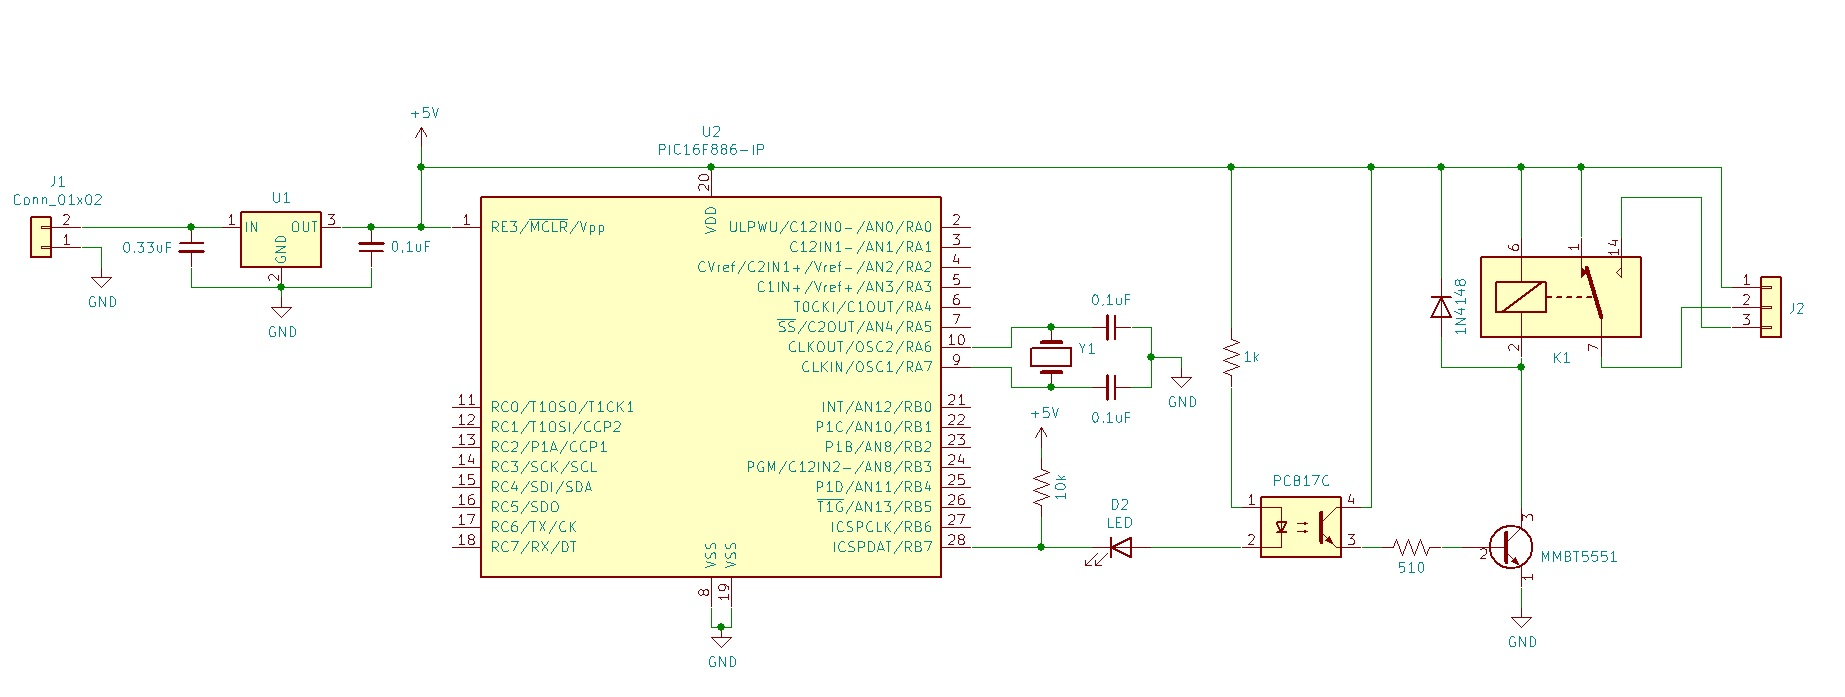
\includegraphics[width=\textwidth]{imagenes/fig1.jpg} 
	\caption{Esquemático del circuito a analizar}\label{fig:fig1}
 \end{center}
\end{figure}
%
\subsection{Lista de Componentes}
Se presenta la lista de componentes que procederemos a analizar secciones mas adelante: \\
\begin{center}
\begin{tabular}{ | c | c | }
  \hline
  Dispostivo & Cantidad \\
  \hline 
    Capacitor 0,1 uF & 3  \\
  \hline 
    Capacitor 0,33 uF & 1  \\
  \hline 
    Regulador de tensión LM7805& 1  \\
  \hline 
    Microcontrolador 16F886 & 1  \\
  \hline
    Cristal  & 1  \\
  \hline
    Resistencias SMD & 3  \\
  \hline
    Diodo LED  & 1  \\
  \hline
    Diodo 1N4148 & 1  \\
  \hline
    Optoacoplador PC817C  & 1  \\
  \hline
    Relé electromecánico  & 1  \\
  \hline
\end{tabular}
\end{center}

\section{Norma MIL-HDBK-217F}
El propósito de este manual es establecer y mantener métodos consistentes y uniformes para estimar la confiabilidad inherente de equipos y sistemas electrónicos militares. Bajo esta norma se establece el tiempo medio entre fallas (MTBF) de dos maneras diferentes, primero se hace el cálculo con respecto al \textit{análisis por stress} el cual tiene en cuenta numerosos parámetros que afectan la vida útil de los componetes, dando como resultado una aproximación mas acertada a la vida útil global, y luego se emplea el método de \textit{cuenta partes} el cual necesita menos información pero tiene la ventaja que es mas generalizado y de mas rápida elaboración.

\subsection{Análisis por Stress}
El método de análisis por stres de la pieza se usa la mayoría del tiempo y es aplicable cuando el diseño está casi terminado y hay una lista detallada de piezas, o BOM, además de la disponibilidad del stress de los componentes. Por stress de componentes, la norma se refiere a las condiciones de operación reales, como el ambiente, la temperatura, la tensión, la corriente y los niveles de potencia aplicados, por ejemplo. El estándar MIL-217 agrupa componentes o partes por categorías principales y luego tiene subgrupos dentro de las categorías. Cada componente o categoría de pieza y sus subgrupos tienen una fórmula o modelo único aplicado para calcular la tasa de falla de ese componente o pieza.

Se desarrollaran cada uno de los componentes, teniendo en cuenta a qué grupo pertenece y su respectiva fórmula para obtener la probabilidad de falla $\lambda_P$ cuya unidad es fallas con respecto a un millón de horas. Con este calculado se procede a calcular el tiempo medio entre fallas o tiempo medio de vida (MTFB) de acuerdo a la siguiente ecuación \ref{eq:lambda}, la cual aplica tanto para elementos individuales o sistemas.

\begin{equation}
MTFB \; = \frac{1}{\lambda_P} \; [Hs] \label{eq:lambda}
\end{equation}

\subsubsection{Diodo 1N4148}
Se calcula de la siguiente manera:

\[\lambda_P = \lambda_b  \cdot \pi_T  \cdot \pi_Q  \cdot \pi_C  \cdot  \pi_S \] 

\begin{center}
\begin{tabular}{ | c | c | c | c | c | c | c | }
  \hline
  Modelo & $\lambda_b$ & $\pi_T$ & $\pi_Q$ & $\pi_C$ &  $\pi_S$ & $\lambda_P$ \\
  \hline
    1N4148 & 0,013 & 32 & 8,0 & 1 &  0,054 & \num{2,2464e-3} \\
  \hline
 \end{tabular}
\end{center}
 
\subsubsection{Transistor Bipolar MMBT5551}
Se calcula de la siguiente manera:

\[\lambda_P = \lambda_b  \cdot \pi_T  \cdot \pi_A  \cdot \pi_R  \cdot \pi_S  \cdot  \pi_Q  \cdot  \pi_E \] 

\begin{center}
\begin{tabular}{ | c | c | c | c | c | c | c | c |  c | }
  \hline
  Modelo & $\lambda_b$ & $\pi_T$ & $\pi_A$ & $\pi_R$ & $\pi_S$ &  $\pi_Q$ &  $\pi_E$  & $\lambda_P$ \\
  \hline
    MMBT5551 & 0,00074 & 8,1 & 0,70 & 0,43 &  0,00142 & 1,0 & 5,5 &  \num{1,409e-5} \\
  \hline
\end{tabular}
\end{center}

\subsubsection{Optoacoplador Pc817c }
Se calcula de la siguiente manera:

\[\lambda_P = \lambda_b  \cdot \pi_T  \cdot \pi_Q  \cdot \pi_E \] 
\begin{center}
\begin{tabular}{ | c | c | c | c | c | c |}
  \hline
  Modelo & $\lambda_b$ & $\pi_T$ & $\pi_Q$ & $\pi_E$ & $\lambda_P$ \\
  \hline
    PC817C & 0,013 & 6,3 & 5,5 & 1,0 &  0,45 \\
  \hline
\end{tabular}
\end{center}

\subsubsection{Relé Electromecánico SRD-05VDC-SL}
Se calcula de la siguiente manera:

\[\lambda_P = \lambda_b  \cdot \pi_L  \cdot \pi_C  \cdot \pi_{CYC}  \cdot \pi_F  \cdot \pi_Q  \cdot \pi_E \] 

\begin{center}
\begin{tabular}{ | c | c | c | c | c | c | c | c | c |}
  \hline
  Modelo & $\lambda_b$ & $\pi_L$ & $\pi_C$ & $\pi_{CYC}$ & $\pi_F$ & $\pi_Q$ & $\pi_E$ & $\lambda_P$ \\
  \hline
    SRD-05VDC-SL & 0,0061 & 0,7 & 1,75 & 1,0 & 1,5 & 8 & 2,0 & 0,17 \\
  \hline
\end{tabular}
\end{center}

\subsubsection{LED SMD VLMW11R2S2}
Se calcula de la siguiente manera:

\[\lambda_P = \lambda_b  \cdot \pi_T  \cdot \pi_Q  \cdot \pi_E \] 
\begin{center}
\begin{tabular}{ | c | c | c | c | c | c |}
  \hline
  Modelo & $\lambda_b$ & $\pi_T$ & $\pi_Q$ & $\pi_E$ & $\lambda_P$ \\
  \hline
    VLMW11R2S2 & 0,00023 & 5,3 & 5,5 & 1,0 & \num{6,7045e-3} \\
  \hline
\end{tabular}
\end{center}

\subsubsection{Resistores}
Se calcula de la siguiente manera:

\begin{center}
\begin{tabular}{ | c | c | c | c | c | c |}
  \hline
  Modelo & $\lambda_b$ & $\pi_{R}$ & $\pi_Q$ & $\pi_E$ & $\lambda_P$ \\
  \hline
    1 k$\Omega$ & 0,00022 & 1,0 & 15 & 1,0 & \num{3,3e-3} \\
  \hline
    10 k$\Omega$ & 0,00022 & 1,0 & 15 & 1,0 & \num{3,3e-3} \\
  \hline
    510 $\Omega$ & 0,00031 & 1,0 & 15 & 1,0 & \num{4,65e-3} \\
  \hline
\end{tabular}
\end{center}

\subsubsection{Capacitores}
Se calcula de la siguiente manera:

\[ \lambda_P = \lambda_b  \cdot \pi_{Cv}  \cdot \pi_Q  \cdot \pi_E \] 

\begin{center}
\begin{tabular}{ | c | c | c | c | c | c |}
  \hline
  Modelo & $\lambda_b$ & $\pi_{Cv}$ & $\pi_Q$ & $\pi_E$ & $\lambda_P$ \\
  \hline
    0,33 uF & 0,00097 & 0,29 & 7,0 & 1,0 & \num{1,96e-3} \\
  \hline
    0,1  uF & 0,00097 & 0,259 & 7,0 & 1,0 & \num{1,75e-3} \\
  \hline
\end{tabular}
\end{center}

\subsubsection{Microcontrolador 16F886}
Se calcula de la siguiente manera:

\[\lambda_P = (C_1  \cdot \pi_T + C_2  \cdot \pi_E)  \cdot \pi_Q \cdot \pi_L \] 

\begin{center}
\begin{tabular}{ | c | c | c | c | c | c | c | c |}
  \hline
  Modelo & $C_1$ & $\pi_T$ & $C_2$ & $\pi_E$ & $\pi_Q$ & $\pi_L$ & $\lambda_P$ \\
  \hline
    16F886 & 0,14 & 5,5 & 0,0014 & 0,5 & 1 & 1,0 & 0,7707 \\
  \hline
\end{tabular}
\end{center}

\subsubsection{Cristal de Quarzo}
Se calcula de la siguiente manera:

\[\lambda_P = \lambda_b  \cdot \pi_Q  \cdot \pi_E \] 
\begin{center}
\begin{tabular}{ | c | c | c | c | c |}
  \hline
  Modelo & $\lambda_b$ & $\pi_Q$ & $\pi_E$ & $\lambda_P$ \\
  \hline
    8Mhz & 0,022 & 2,1 & 1,0 & 0,0462 \\
  \hline
\end{tabular}
\end{center}

\subsubsection{Regulador de Tensión LM7805}
Se calcula de la siguiente manera:

\[\lambda_P = (C_1  \cdot \pi_T + C_2  \cdot \pi_E)  \cdot \pi_Q  \cdot \pi_L \] 

\begin{center}
\begin{tabular}{ | c | c | c | c | c | c | c | c |}
  \hline
  Modelo & $C_1$ & $\pi_T$ & $C_2$ & $\pi_E$ & $\pi_Q$ & $\pi_L$ & $\lambda_P$ \\
  \hline
    LM7805 & 0,010 & 180 & 0,00027 & 0,5 & 0,25 & 1,0 & 0,0453375 \\
  \hline
\end{tabular}
\end{center}

\subsubsection{$\lambda_{pT}$ del sistema}
A partir de cada $\lambda_P$ se puede obtener el  $\lambda_{pT}$ del sistema mediante la sumatoria de cada uno de ellos multiplicado por un factor $n$ correspondiente a la cantidad de veces que se repite, de modo que:

\begin{align*}
\lambda_{pT} =&\lambda_{C0,33uF} + 3 \cdot \lambda_{C0,1uF} + \lambda_{LM7805} \; + \lambda_{Crystal} \;+\; \lambda_{16F886} \;+\; \lambda_{R10k} \;+\;\\
			  &\lambda_{R1k} \;+\; \lambda_{R510} \;+\; \lambda_{1N4148} \;+\; \lambda_{rele} \;+\; \lambda_{BJT} \;+\; \lambda_{optoacoplador} \;+\; \lambda_{LED} \\
\lambda_{pT} =&1,85437049 
\end{align*}

Quedando finalmente como vida media:

\begin{align*}
{MTBF}\bigr|_{Sistema} 	&= \frac{\num{e6}}{\lambda_{pT}} \\
						&= \frac{\num{e6}}{1,85437049 } \\
						&= 39266,5626  \; [Hs] \\
						&= 22469,44  \;   [Dias] \\
{MTBF}\bigr|_{Sistema}	&= 615,60 \;  [A\tilde{n}os] 
\end{align*}

Esto indica que nuestro circuito tiene una vida media de aproximadamente 62 años, puede durar más o menos, pero nos da la certeza que  la probabilidad de falla de la mayoría de nuestros circuitos oscilará en un período de 62 años.

\subsection{Análisis por cuenta partes}
El método de análisis de cuentas partes requiere menos información,tal como cantidades de piezas, nivel de calidad y entorno de aplicación. Es más aplicable durante las fases iniciales de diseño o propuesta de un proyecto. 

El estándar MIL-217 proporciona tablas para los grupos de componentes (los mismos grupos que el análisis por stress) que enumeran las tasas de falla y los factores de calidad genéricos para los diferentes entornos MIL-217.

El análisis de recuento de piezas no tiene en cuenta las numerosas variables y utiliza las tasas de falla genéricas o de base más desfavorables y los factores $\pi$. El Método de cuenta de partes generalmente resultará en una mayor tasa de fallas o en una menor confiabilidad del sistema, lo que brinda un resultado más conservador que el que generaría el método de stress.

Para este cálculo se utiliza la siguiente ecuación:
\begin{equation}
	\lambda_{Pequip} = \sum_{1}^{n} i N_i  \cdot (\lambda_g  \cdot \pi Q) i
\end{equation}

\begin{center}
\begin{tabular}{| c | c | c | c | c | c |}
\hline
Componentes & $N_i$ & $\lambda_g$ & $\pi Q$ & $\lambda_p$ & MTBF [Hs] \\
\hline
LM7805 & 1 & 0,0036 & 0,25 & \num{9e-4} & 2205979,625 \\
\hline
Capacitor cerámico & 4 & 0,0036 & 10 & 0,144 & 69444444,44 \\
\hline
Cristal Quarzo & 1 & 0,0032 & 2,1 & \num{6,32e-3} & 1488095238 \\
\hline
Microcontrolador & 1 & 0,048 & 0,25 & 0,012 & 833333333,3 \\
\hline
Resistencia carbon & 3 & 0,0019 & 10 & 0,057 & 175438596,5 \\
\hline
LED & 1 & 0,00047 & 5,5 & \num{2,5855e-3} & 3868471954 \\
\hline
Optoacoplador & 1 & 0,027 & 5,5 & 0,1485 & 67340067,34 \\
\hline
BJT & 1 & 0,00015 & 5,5 & \num{8,25e-4} & \num{1,21e10} \\
\hline
Rele & 1 & 0,13 & 9,0 & 1,17 & 8547008,547 \\
\hline
Diodo 1N4148 & 1 & 0,0029 & 5,5 & 0,01595 & 626959247,6 \\
\hline
\multicolumn{4}{|c|}{$\lambda_{Pequi}$} & 1,5580805 & 6418453,619\\
\hline
\end{tabular}
\end{center}

como previamente se hizo con la ecuación \ref{eq:lambda},
\begin{align*}
{MTBF}\bigr|_{Sistema} 	&= \frac{\num{e6}}{\lambda_{Pequi}} \\
						&= \frac{\num{e6}}{1,5580805 } \\
						&= 6418453,619  \; [Hs] \\
						&= 267423,06  \;   [Dias] \\
{MTBF}\bigr|_{Sistema}	&= 732,66 \;  [A\tilde{n}os] 
\end{align*}
Aquí se pone en evidencia lo antes expuesto, la vida media difiere ya que los métodos consideran distinta variables, siendo el análisis por stress el más fidedigno, ya que considera mayor cantidad de aspectos reales, aunque para ser un sistema tentativo el método por cuenta partes cumple su función, en nuestro caso expone la longevidad del correcto funcionamiento de nuestro circuito.

\section{Norma MIL-HDBK-338}

\subsection{Análisis del modo de fallas y sus efectos (FMEA)}
El FMEA se define como un procedimiento de confiabilidad en el cual se describe cada falla posible y su efecto en el desempeño final del sistema. Es un análisis a nivel de componente, donde para efectuarse se debe considerar cada falla como la única falla en el sistema. En base al objetivo por el que se busca brindar mayor confiabilidad o seguridad en aquello que se busca proteger, se determina la probabilidad de pérdida de función $\beta$ , según el siguiente criterio:

\begin{table}[h!]
\centering
\begin{tabular}{@{}c|c@{}}
\toprule
\multicolumn{1}{|c|}{Efecto de falla} & \multicolumn{1}{c|}{$\beta$} \\ \midrule
Perdida segura & 1 \\ \midrule
Perdida probable & \textgreater{}0.1 a \textless{}1 \\ \midrule
Posible perdida & \textgreater{}0 a \textless{}0.1 \\ \midrule
Sin efecto & 0 \\ \bottomrule
\end{tabular}
\end{table}

\subsubsection{Tabla de análisis FMEA}

% Please add the following required packages to your document preamble:
% \usepackage{booktabs}
% \usepackage{multirow}
\begin{table}[h!]
\centering
\begin{tabular}{@{}|c|c|c|c|@{}}
\toprule
\textit{Item} & \textit{\textbf{Modos de falla}} & \textit{\textbf{Efecto de la falla}} & \textit{\textbf{$\beta$}} \\ \midrule
\multirow{3}{*}{\textit{\textbf{\begin{tabular}[c]{@{}c@{}}Diodo\\ 1n4148\end{tabular}}}} & Short & \begin{tabular}[c]{@{}c@{}}Aumento $I_{C2}$\\ No activa Relay\end{tabular} & 1 \\ \cmidrule(l){2-4} 
 & Open & No elimina transistorios & 0.1 \\ \cmidrule(l){2-4} 
 & Cambio de parámetros & Puede Quemarse & 0.1 \\ \midrule
\multirow{2}{*}{\textbf{LED}} & Short & Cambio de corriente entrada al optoacoplador & 0.1 \\ \cmidrule(l){2-4} 
 & Open & No activa optoacoplador & 1 \\ \midrule
\multirow{3}{*}{\textbf{Relay}} & Fails to trip & No activa salida & 1 \\ \cmidrule(l){2-4} 
 & Spurius trip & No activa salida & 1 \\ \cmidrule(l){2-4} 
 & Short & No activa salida & 1 \\ \midrule
\multirow{3}{*}{\textbf{\begin{tabular}[c]{@{}c@{}}Resistencia\\ $1 k \Omega$\end{tabular}}} & Short & Posible exceso de corriente de entrada opto & 1 \\ \cmidrule(l){2-4} 
 & Open & No activa salida & 1 \\ \cmidrule(l){2-4} 
 & Cambio parámetros & Cambia corriente y tensión de entrada de optoacoplador & 1 \\ \midrule
\multirow{3}{*}{\textbf{\begin{tabular}[c]{@{}c@{}}Resistencia\\ $510 \Omega$\end{tabular}}} & Short & Posible exceso de $I_{B2}$ & 0.1 \\ \cmidrule(l){2-4} 
 & Open & No saturación transistor & 1 \\ \cmidrule(l){2-4} 
 & Cambio de parámetros & Posible exceso de $I_{B2}$ & 0.1 \\ \midrule
\multirow{3}{*}{\textbf{\begin{tabular}[c]{@{}c@{}}Resistencia \\ $10 k \Omega$\end{tabular}}} & Short & Posible perdida de puerto de salida microcontrolador & 1 \\ \cmidrule(l){2-4} 
 & Open &  & 0 \\ \cmidrule(l){2-4} 
 & Cambio de parámetros & Posible ruido & 0.1 \\ \midrule
\multirow{2}{*}{\textbf{Transistor bipolar}} & Open & No saturació salida & 1 \\ \cmidrule(l){2-4} 
 & Short & Posible activacion de relay & 0.1 \\ \midrule
\multirow{2}{*}{\textbf{Optoacoplador}} & Open & No activa salida & 1 \\ \cmidrule(l){2-4} 
 & Short & Salida siempre en encendida & 1 \\ \bottomrule
\end{tabular}
\end{table}
\clearpage


% Please add the following required packages to your document preamble:
% \usepackage{booktabs}
% \usepackage{multirow}
\begin{table}[h!]
\centering
\begin{tabular}{@{}|c|c|c|c|@{}}
\toprule
\textit{\textbf{Item}} & \textit{\textbf{Modos de falla}} & \textit{\textbf{Efecto de la falla}} & \textit{\textbf{$\beta$}} \\ \midrule
\multirow{3}{*}{\textit{\textbf{\begin{tabular}[c]{@{}c@{}}Regulador de voltaje\\ (7805)\end{tabular}}}} & Open & No activa circuito & 1 \\ \cmidrule(l){2-4} 
 & Short & Perdida del sistema & 1 \\ \cmidrule(l){2-4} 
 & Cambio de parámetros & Posible falla del sistema & 0.1 \\ \midrule
\multirow{3}{*}{\textbf{\begin{tabular}[c]{@{}c@{}}Capacitores\\ $C_1$ y $C_2$\end{tabular}}} & Open & 7805 no estable & 0.1 \\ \cmidrule(l){2-4} 
 & Short & 7805 no estable & 0.1 \\ \cmidrule(l){2-4} 
 & Cambio de parámetros & 7805 no estable & 0.1 \\ \midrule
\multirow{3}{*}{\textbf{\begin{tabular}[c]{@{}c@{}}Capacitores\\ $C_3$ y $C_4$\end{tabular}}} & Open & Oscilador no estable & 1 \\ \cmidrule(l){2-4} 
 & Short & Oscilador & 1 \\ \cmidrule(l){2-4} 
 & Cambio de parámetros & Oscilador & 1 \\ \midrule
\multirow{4}{*}{\textbf{Cristal}} & Output depraded & Incorrecto funcionamiento de microcontrolador & 1 \\ \cmidrule(l){2-4} 
 & No output & No funcionamiento de microcontrolador & 1 \\ \cmidrule(l){2-4} 
 & Fails to run after start & No funcionamiento de microcontrolador & 1 \\ \cmidrule(l){2-4} 
 & Loss of control & No funcionamiento de microcontrolador & 1 \\ \midrule
\multirow{5}{*}{\textbf{\begin{tabular}[c]{@{}c@{}}PIC \\ Microcontrolador\\ digital CMOS\end{tabular}}} & Input open & Posible mal funcionamiento & 0.1 \\ \cmidrule(l){2-4} 
 & Output open & No activa salida & 1 \\ \cmidrule(l){2-4} 
 & Supply open & No activa salida & 1 \\ \cmidrule(l){2-4} 
 & Output stay low & No activa salida & 1 \\ \cmidrule(l){2-4} 
 & Output stay high & Incorrecta activación salida & 1 \\ \bottomrule
\end{tabular}
\end{table}


\subsection{Análisis del Árbol de Fallas (FTA)}

Es un procedimiento de confiabilidad donde se analiza a partir desde cada falla posible a la salida del sistema y se procede a identificar sus causas hacia los componentes del sistema. Es un análisis a nivel de sistema, el cuál
se realiza mediante un diagrama de bloques de falla/avería, identificando la falla principal del sistema y se la relaciona en orden descendente con las posibles causas, las cuales pueden ser la avería de algún componente o alguna falla previa.

Para el circuito bajo estudio, se presentaran dos situaciones de fallos, la primera es la que la salida se mantiene en alto y la segunda es el caso contrario, las salidas permanecen en bajo.

\begin{figure}[h!]
	\centering
	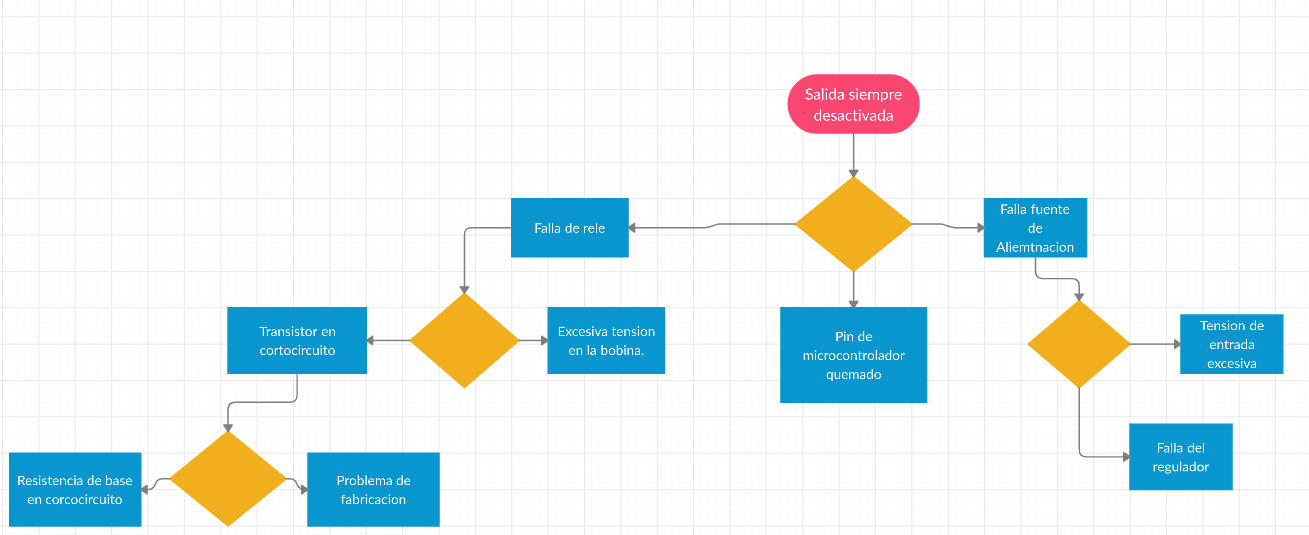
\includegraphics[width=\textwidth]{imagenes/Arbol2.png}
	\caption{Salida siempre desactivada}
\end{figure} 

\begin{figure}[h]
	\centering
	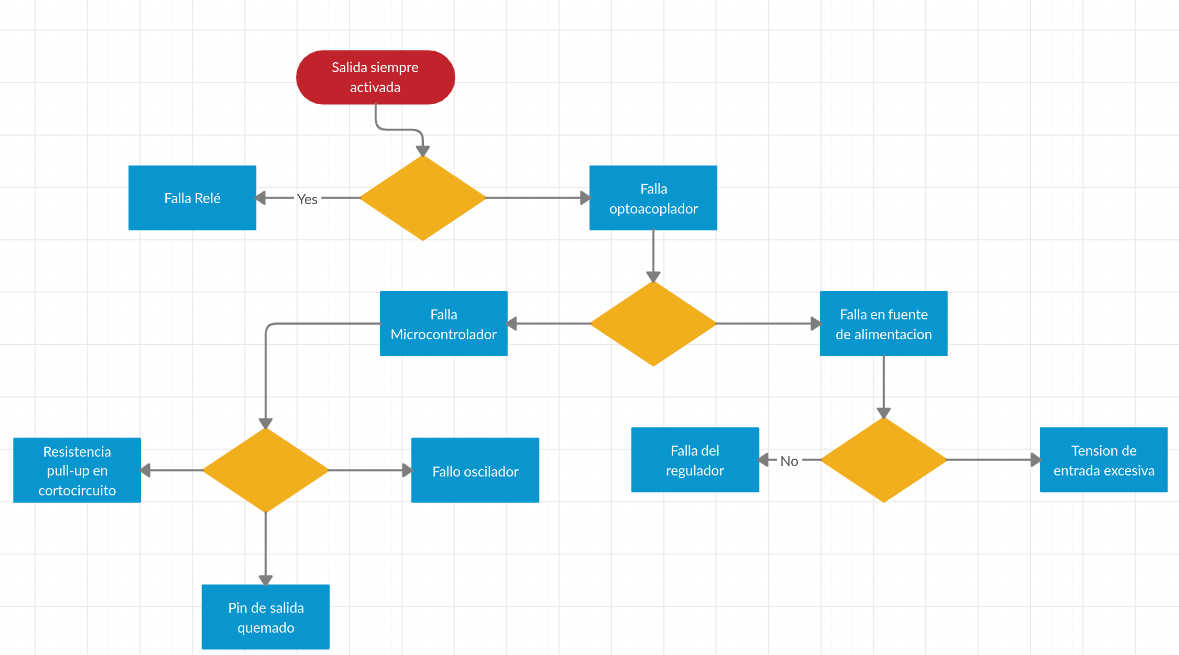
\includegraphics[width=\textwidth]{imagenes/Arbol1.png}
	\caption{Salida siempre activada}
\end{figure} 

\subsection{Análisis Crítico de Modo de Fallas (FMECA)}

Procedimiento de confiabilidad donde, a partir del FMEA, se jerarquiza cada falla según categorías de efecto de falla y probabilidad de ocurrencia. De esta manera se identifican los puntos simples de falla que resultan críticos para lograr un diseño confiable o para crear seguridad. Esto último se debe interpretar en relación a lo que se está buscando proteger, ya sea al usuario, medio ambiente, un sistema previo, etc. 

Este análisis se basa en:

\begin{itemize}
	\item Determinar el numero critico de modo de falla $C_m$, el cual viene dado por la siguiente ecuación:
		\begin{equation}
			C_m = \beta \cdot \alpha \cdot \lambda_{p} \cdot t
		\end{equation}
	Donde cada coeficiente es:
	\begin{itemize}
	  \item $\beta$ : Probabilidad de pérdida de función.
	  \item $\alpha$ : Probabilidad de modo de falla.
	  \item $\lambda_{p}$ : probabilidad de falla total.
	  \item $t$ : tiempo de funcionamiento requerido.
	\end{itemize}
	
  \item A partir de este se puede determinar la criticidad total del sistema como:
  \begin{equation}
	  C_{r_{TOTAL}} = \sum{c_m} 
  \end{equation}
 
  \item Determinar el numero critico de cada item $C_T$ como:
	  \begin{equation}
		  C_r = \sum_{n=1}^{j}{(C_m)_n}
	  \end{equation}
	  Siendo $j$ el numero de modos de fallas del item o componente.

  \item	Clasificar a cada modo de falla en base a ka categoría de gravedad, según lo que se busca proteger, y probabilidad de ocurrencia según los siguientes criterios:

\begin{table}[h]
\centering
\begin{tabular}{@{}|c|c|@{}}
\toprule
\textit{\textbf{Criterio de gravedad}} & \textit{\textbf{Tipo}} \\ \midrule
I & Catastrófico \\ \midrule
II & Importante \\ \midrule
II & Marginal \\ \midrule
IV & Menor \\ \bottomrule
\end{tabular}
\end{table}

% Please add the following required packages to your document preamble:
% \usepackage{booktabs}
\begin{table}[H]
\centering
\begin{tabular}{@{}|c|c|@{}}
\toprule
\textit{\textbf{Probabilidad de ocurrencia}} & \textit{\textbf{Frecuencia}} \\ \midrule
Nivel A & Frecuente \\ \midrule
Nivel B & Razonablemente probable \\ \midrule
Nivel C & Ocasional \\ \midrule
Nivel D & Remota \\ \midrule
Nivel E & Improbable \\ \bottomrule
\end{tabular}
\end{table}

\item Construir una matriz de criticidad, en base a los números críticos, categoría de gravedad y probabilidad de ocurrencia.
\end{itemize}

A continuación se muestran los resultados del análisis del FMECA correspondiente al circuito.


% Please add the following required packages to your document preamble:
% \usepackage{booktabs}
% \usepackage{multirow}
% \usepackage{graphicx}
\begin{table}[H]
\centering
\resizebox{\textwidth}{!}{%
\begin{tabular}{@{}|c|c|c|c|c|c|c|c|@{}}
\toprule
\textbf{Componente} & \textbf{\begin{tabular}[c]{@{}c@{}}Prob. modo de falla\\ $\alpha$\end{tabular}} & \textbf{\begin{tabular}[c]{@{}c@{}}Prob. perdida de funcion\\ $\beta$\end{tabular}} & \textbf{\begin{tabular}[c]{@{}c@{}}Prob. falla de componente\\ $\lambda_{p}$\end{tabular}} & \textbf{\begin{tabular}[c]{@{}c@{}}$C_m$ \\ $\frac{fallas}{10}^6$\end{tabular}} & \textbf{\begin{tabular}[c]{@{}c@{}}$C_r$\\ $\frac{fallas}{10}^6$\end{tabular}} & \textbf{Severidad} & \textbf{Prob de ocurrencia} \\ \midrule
\multirow{3}{*}{\textbf{\begin{tabular}[c]{@{}c@{}}Regulador\\ 7805\end{tabular}}} & Open (0.45) & 1 & \multirow{3}{*}{0.453} & 0.204 & \multirow{3}{*}{0.4536} & IV & B \\ \cmidrule(lr){2-3} \cmidrule(lr){5-5} \cmidrule(l){7-8} 
 & Change parameter (0.35) & 0.1 &  & 0.159 &  & III & B \\ \cmidrule(lr){2-3} \cmidrule(lr){5-5} \cmidrule(l){7-8} 
 & Short (0.20) & 1 &  & 0.0906 &  & II & C \\ \midrule
\multirow{3}{*}{\textbf{\begin{tabular}[c]{@{}c@{}}$C_1$\\ (0.3 uF)\end{tabular}}} & Open (0.22) & 0.1 & \multirow{3}{*}{$\num{1.96e-3}$} & $\num{4.321e-5}$ & \multirow{3}{*}{$\num{1.952e-4}$} & III & E \\ \cmidrule(lr){2-3} \cmidrule(lr){5-5} \cmidrule(l){7-8} 
 & Short (0.49) & 0.1 &  & $\num{9.6e-5}$ &  & IV & E \\ \cmidrule(lr){2-3} \cmidrule(lr){5-5} \cmidrule(l){7-8} 
 & Change parameter (0.29) & 0.1 &  & $\num{5.6e-5}$ &  & IV & E \\ \midrule
\multirow{3}{*}{\textbf{\begin{tabular}[c]{@{}c@{}}$C_2$,  $C_3$, $C_4$\\ (0.1 uF)\end{tabular}}} & Open (0.22) & 1 & \multirow{3}{*}{$\num{1.75e-3}$} & $\num{3.85e-4}$ & \multirow{3}{*}{$\num{17.49e-4}$} & IV & E \\ \cmidrule(lr){2-3} \cmidrule(lr){5-5} \cmidrule(l){7-8} 
 & Short (0.49) & 1 &  & $\num{8.57e-4}$ &  & IV & E \\ \cmidrule(lr){2-3} \cmidrule(lr){5-5} \cmidrule(l){7-8} 
 & Change parameter (029) & 1 &  & $\num{5.07e-4}$ &  & IV & E \\ \midrule
\multirow{4}{*}{\textbf{Cristal}} & Output depradated (0.6) & 1 & \multirow{4}{*}{0.0462} & 0.027 & \multirow{4}{*}{0.0453} & III & C \\ \cmidrule(lr){2-3} \cmidrule(lr){5-5} \cmidrule(l){7-8} 
 & No output (0.22) & 1 &  & 0.01 &  & III & C \\ \cmidrule(lr){2-3} \cmidrule(lr){5-5} \cmidrule(l){7-8} 
 & Fails to run (0.09) & 1 &  & $\num{4.158e-3}$ &  & III & D \\ \cmidrule(lr){2-3} \cmidrule(lr){5-5} \cmidrule(l){7-8} 
 & Loss of control (0.09) & 1 &  & $\num{4.158e-3}$ &  & IV & D \\ \midrule
\multirow{5}{*}{\textbf{\begin{tabular}[c]{@{}c@{}}PIC \\ Microcontrolador digital\\ CMOS\end{tabular}}} & Input open (0.36) & 0.1 & \multirow{5}{*}{0.7707} & 0.277 & \multirow{5}{*}{0.774} & IV & A \\ \cmidrule(lr){2-3} \cmidrule(lr){5-5} \cmidrule(l){7-8} 
 & Output open (0.36) & 1 &  & 0.277 &  & III & A \\ \cmidrule(lr){2-3} \cmidrule(lr){5-5} \cmidrule(l){7-8} 
 & Supply open (0.12) & 1 &  & 0.09 &  & III & C \\ \cmidrule(lr){2-3} \cmidrule(lr){5-5} \cmidrule(l){7-8} 
 & Output stack low (0.09) & 1 &  & 0.069 &  & III & C \\ \cmidrule(lr){2-3} \cmidrule(lr){5-5} \cmidrule(l){7-8} 
 & Output stay high (0.08) & 1 &  & 0.061 &  & III & C \\ \midrule
\multirow{3}{*}{\textbf{\begin{tabular}[c]{@{}c@{}}$R_1$\\ $10 k\Omega$\end{tabular}}} & Open (0.66) & 1 & \multirow{3}{*}{$\num{3.3e-3}$} & $\num{2.17e-3}$ & \multirow{3}{*}{3.269} & IV & D \\ \cmidrule(lr){2-3} \cmidrule(lr){5-5} \cmidrule(l){7-8} 
 & Short (0.1) & 0.1 &  & $\num{1e-3}$ &  & IV & D \\ \cmidrule(lr){2-3} \cmidrule(lr){5-5} \cmidrule(l){7-8} 
 & Change parameter (0.03) & 1 &  & $\num{9.9e.5}$ &  & IV & E \\ \midrule
\multirow{3}{*}{\textbf{\begin{tabular}[c]{@{}c@{}}$R_2$\\ $1 k\Omega$\end{tabular}}} & Open (0.31) & 1 & \multirow{3}{*}{$\num{3.3e-3}$} & $\num{1e-3}$ & \multirow{3}{*}{3.269} & III & D \\ \cmidrule(lr){2-3} \cmidrule(lr){5-5} \cmidrule(l){7-8} 
 & Short (0.03) & 1 &  & $\num{9.9e.5}$ &  & II & E \\ \cmidrule(lr){2-3} \cmidrule(lr){5-5} \cmidrule(l){7-8} 
 & Change parameter (0.66) & 1 &  & $\num{2.17e-3}$ &  & IV & D \\ \midrule
\multirow{3}{*}{\textbf{\begin{tabular}[c]{@{}c@{}}$R_3$\\ $510 \Omega$\end{tabular}}} & Open (0.66) & 0.1 & \multirow{3}{*}{$\num{4.65e-3}$} & $\num{3.06e-3}$ & \multirow{3}{*}{$\num{5.895e-3}$} & III & D \\ \cmidrule(lr){2-3} \cmidrule(lr){5-5} \cmidrule(l){7-8} 
 & Short (0.31) & 1 &  & $\num{1.44e-3}$ &  & IV & D \\ \cmidrule(lr){2-3} \cmidrule(lr){5-5} \cmidrule(l){7-8} 
 & Change parameter (0.03) & 0.1 &  & $\num{1.395e-3}$ &  & II & D \\ \midrule
\multirow{2}{*}{\textbf{LED}} & Open (0.7) & 1 & \multirow{2}{*}{$\num{6.7e-3}$} & $\num{4.69e-3}$ & \multirow{2}{*}{$\num{6.1e-3}$} & III & D \\ \cmidrule(lr){2-3} \cmidrule(lr){5-5} \cmidrule(l){7-8} 
 & Short (0.3) & 0.1 &  & $\num{2.01e-3}$ &  & III & D \\ \midrule
\multirow{2}{*}{\textbf{Optoacoplador}} & Open (0.27) & 1 & \multirow{2}{*}{0.45} & 0.1215 & \multirow{2}{*}{0.45} & III & B \\ \cmidrule(lr){2-3} \cmidrule(lr){5-5} \cmidrule(l){7-8} 
 & Short (0.73) & 1 &  & 0.3285 &  & III & A \\ \midrule
\multirow{2}{*}{\textbf{BJT}} & Open (0.27) & 1 & \multirow{2}{*}{$\num{1.4e-5}$} & $\num{3.78e-6}$ & \multirow{2}{*}{$\num{3.8822e-6}$} & III & E \\ \cmidrule(lr){2-3} \cmidrule(lr){5-5} \cmidrule(l){7-8} 
 & Short (0.73) & 0.1 &  & $\num{1.022e-5}$ &  & III & E \\ \midrule
\multirow{3}{*}{\textbf{Relay}} & Fails to trip (0.55) & 1 & \multirow{3}{*}{0.17} & 0.0935 & \multirow{3}{*}{0.17} & IV & C \\ \cmidrule(lr){2-3} \cmidrule(lr){5-5} \cmidrule(l){7-8} 
 & Spurius trip (0.29) & 1 &  & 0.0442 &  & IV & C \\ \cmidrule(lr){2-3} \cmidrule(lr){5-5} \cmidrule(l){7-8} 
 & Short (0.19) & 1 &  & 0.323 &  & IV & A \\ \midrule
\multirow{3}{*}{\textbf{1n4146}} & Open (0.51) & 0.1 & \multirow{3}{*}{$\num{2.24e-3}$} & $\num{1.14e-3}$ & \multirow{3}{*}{$\num{2.22e-3}$} & IV & D \\ \cmidrule(lr){2-3} \cmidrule(lr){5-5} \cmidrule(l){7-8} 
 & Short (0.29) & 1 &  & $\num{6.49e-4}$ &  & III & E \\ \cmidrule(lr){2-3} \cmidrule(lr){5-5} \cmidrule(l){7-8} 
 & Change parameter (0.2) & 0.1 &  & $\num{4.4e-4}$ &  & IV & E \\ \bottomrule
\end{tabular}%
}
\end{table}

\clearpage

\subsubsection {Matriz de Criticidad}

\begin{figure}[h]
 \centering
	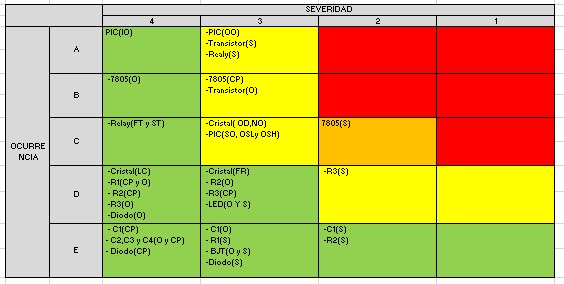
\includegraphics[width=\textwidth]{imagenes/matriz.jpeg} 
	\caption{Matriz de criticidad}
\end{figure}

Donde:
\begin{itemize}
	\item LC : Loss of control.
	\item O : Open.
	\item S : Short.
	\item CP : Change parameter.
	\item NO : No output.
	\item OD : Output degradated.
	\item FR : Fail to run.
	\item IO : Input Open.
	\item OO : Output open.
	\item SO : Supply open.
	\item OSL : Output stuck low.
	\item OSH : Output stuck high.
	\item FT : Fails to trip.
	\item ST : Spurius Trip.
\end{itemize}
\clearpage

\subsection {Conclusiones}

\begin{itemize}
	\item El objetivo de estos análisis es estimar la vida útil de sistemas electrónicos a diseñar/realizar y poder tener una estimación de su calidad, puntos débiles en el diseño y tiempo entre reparaciones, y si es un producto comercial garantizar un periodo de funcionamiento al cliente.

\item El análisis por cuenta partes es mucho mas sencillo y rápido de realizar que el análisis por estrés, quedando el primero relegado solo a una fase de diseño a desarrollar, es útil para tener una estimación temprana de si el diseño cumple con los requerimientos impuestos, ya sea por el diseñador o la que especifique la norma que aplica al sistema.

	\item Tanto el árbol de fallas como la matriz de criticidad son métodos muy útiles, ya que con simples gráficos se pueden saber las posibles fallas y sus correspondientes causas, y los eslabones críticos del circuito electrónico, respectivamente. Son dos gráficos que sus informaciones se corresponden, ya que los mayores causantes de las principales fallas los generan los dispositivos más probables a fallar. 


  \item Se corroboró la importancia a nivel práctica profesional de estos análisis. Desde un pequeño circuito como podría ser el elegido en este trabajo práctico hasta en grandes fabricas, como por ejemplo, en una linea robotizada, son necesarios los cálculos de confiabilidad. De esta manera se tiene información de qué puede fallar, en cuánto tiempo y por sobretodo actuar ante estas fallas.
\end{itemize}

\end{document}
